\documentclass[12pt,letterpaper]{article}

\PassOptionsToPackage{hyphens}{url}
\usepackage[
  pdftex, 
  bookmarksopen=true, 
  bookmarksnumbered=true,
  pdfstartview=FitH, 
  breaklinks=true, 
  urlbordercolor={0 1 0}, 
  citebordercolor={0 0 1}]
  {hyperref}

\usepackage{setspace}
\onehalfspacing

% === MARGINS ===
\addtolength{\hoffset}{-0.75in} 
\addtolength{\voffset}{-1.25in}
\addtolength{\textwidth}{1.5in} 
\addtolength{\textheight}{2.25in}

% == ENVS ==
\newenvironment{tightcenter}{%
  \setlength\topsep{0pt}
  \setlength\parskip{0pt}
  \begin{center}
}{
  \end{center}
}

% == PACKS ==
\usepackage{color,soul}
\usepackage{graphicx} % to use pngs in tex (include graphix)
\usepackage{calc} % To scale \pagewidth with \real{float}
\usepackage{pgfplots} % To draw histogram
\pgfplotsset{compat=1.17} % request specific version of pgfplots
\usepackage{calc} % to use \real for text -> numeric
\usepackage{pgf} % to store numeric variables
\usepackage{subcaption} % to place two figures horizontally
\usepackage{caption} % to refer subfigure
\renewcommand{\thesubfigure}{(\alph{subfigure})}
\captionsetup[sub]{labelformat=simple}

\usepackage{tikz}
\usetikzlibrary{automata,positioning}
\usetikzlibrary{arrows.meta, positioning, automata}
\usetikzlibrary{spy}

\tikzset{
  font={\fontsize{10pt}{0}\selectfont}}
\usepackage{forest}
\tikzset{
  Decision/.style = {%
    draw,
    line width=1.4pt
  },
  Lottery/.style = {%
    draw,
    line width=1.4pt
  },
  Outcome/.style = {%
    circle,
    minimum width=3pt,
    fill,
    inner sep=0pt
  }
}
\usepackage{csquotes}
\usepackage{lipsum}
\usetikzlibrary{arrows.meta,automata,positioning} % to draw directed-weighted-graph


\usepackage{amsmath, amssymb, latexsym} % NN
\usepackage{tikz}% NN
\usetikzlibrary{decorations.pathreplacing}% NN
\usetikzlibrary{fadings}% NN


\usepackage{xltabular}
\usepackage{booktabs}

\usepackage[breakable]{tcolorbox} % to add factual asepct inside a frame

\usepackage[title]{appendix}

% == Checkmarks == 
\usepackage{bbding}
\usepackage{pifont}
\usepackage{wasysym}
\usepackage{amssymb}
% ================

% == BIBS ==
\usepackage{natbib}

\usepackage{diagbox}

\bibliographystyle{apsr}


% == SPACES == 

% == CMMDS ==
\newcommand{\tit}{
\bf 
Mapping Regulatory Network of WTO Dispute Settlement Body Using Deep Learning
}
\newcommand\spacingset[1]{\renewcommand{\baselinestretch}
{#1}\small\normalsize}

% == VARS == 
\pgfmathsetmacro{\heatmap}{1}

% == START (PageCounter, Mode)
\begin{document}

\spacingset{1.25}

\setcounter{page}{0}
\vspace{-.1in}

% == TITLE (includes DraftDate)
{\title{
    \tit
  }
  \author{Suyeol Yun
  }
  \maketitle
}

\thispagestyle{empty}
\vspace{-.1in}

\begin{abstract}
  % \lipsum[1]
\end{abstract}

\spacingset{1.5} % gives a slightly more margin between abstract and introduction

% \section{Tree of Contents}
% \begin{forest}
        for tree={
          grow=0,
          Decision,
          calign angle=30,
          calign=fixed edge angles,
        }
        [A
          [B, calign secondary angle=0, calign primary angle=-60
            [D]
            [E]
          ]
          [C, calign secondary angle=70, calign primary angle=-60
            [F]
            [G]
          ]
        ]
\end{forest}
      
% \clearpage


\section{Introduction}

The Dispute Settlement Body (DSB) of
the World Trade Organization (WTO) deals
with trade disputes between WTO members.
WTO members file a lawsuit in WTO DSB to
claim their impaired benefit related to the WTO agreements as a result of another member's possible illegal trade policy.
The judicial body of WTO DSB, \textit{Panel} or \textit{Appellate Body}, then adjudicates the dispute and submits a report in which it expresses
its judicial opinion as to whether the challenged
trade policy is inconsistent to the rules of the WTO or not \citep{world2017handbook}.


This process requires enormous legal knowledge and resources because the legal system of WTO is highly complex.
This complexity has constrained many developing countries with limited legal knowledge and resources from fully utilizing the WTO DSB
\citep{busch_reinhardt_shaffer_2009, dev_busch, shaffer_2006}. 
 
To address this issue, I provide a novel method to summarize the network of WTO articles.
Currently, understanding of how articles of WTO agreements systematically interact with each other is exclusively shared among legal experts.
However, by developing the method that can quantitatively summarize the systematic interaction between articles of WTO,
we can lower the cost of understanding the legal system of WTO. This will help resolve the unbalanced legal capacity issue in WTO DSB.
 
To properly summarize the systematic interactions between articles of WTO agreements, I designed my method based on two following considerations.
First, since the legal system of WTO evolves from the way how real-world dispute interacts with the regulatory content of the article of WTO agreement,
I considered a way of utilizing two different types of textual data, factual description of the trade dispute and the content of each article of the WTO agreements.
Second, since members strategically cite rules of the WTO agreements to encourage
the third party participation \citep{who_gets} or to reshape the legal precedents\citep{pelc, latent},
I considered a way of generalizing these member-specific strategic citations.
 
Upon these two considerations, this paper uses deep learning.
Deep learning is empirically known as good at extracting information from the textual data.
In addition to it, deep learning also generalizes the patterns inside data.
Therefore, this paper designs a deep neural network that
processes two different types of textual data,
description of the dispute and each article content of the WTO agreements.
The design mimics the reasoning process of the legal experts,
where the experts read
the textual description of the dispute and imagine applicable legal articles of the WTO agreements according to its regulatory content.
 
To train this neural network, I collected textual description of trade dispute and articles of the WTO agreement cited for each dispute requested to the WTO DSB
from 1995 to 2018.
Using this collected data, I trained the neural network by enforcing the neural network to answer correctly
whether a given article of the WTO agreements
can be cited for the given textual description of
trade dispute.
After training, I fitted a network that summarizes the systematic interactions between articles of WTO agreements using \textit{Random Forests} \citep{rf, genie3}.
The network is fitted as to best explain the variance of each article's citabilities. Those citabilities are collected from the predictions of the trained deep neural network.
 
To verify the quality of the fitted network, I compared the fitted network with the jurisprudence of WTO DSB appearing in the Panel and Appellate Body reports.
Specifically, I found three major principles of WTO DSB, \textit{Market Access}, \textit{Reciprocity}, and \textit{Non-discrimination}, are clustered in the fitted network.
The systematic interactions between articles of WTO agreements are formed as how the Panel and Appellate Body explained in their judicial opinions.
As Panel and Appellate Body authoritatively constitute the jurisprudence of WTO DSB, one can conclude that the method qualitatively summarizes the systematic interactions of articles of WTO agreements.
 
% % == DEF EXAMPLE == 
\begin{figure}[t!]
  \captionsetup[subfigure]{justification=centering}
  \begin{subfigure}[b]{1\textwidth}
      \centering{
              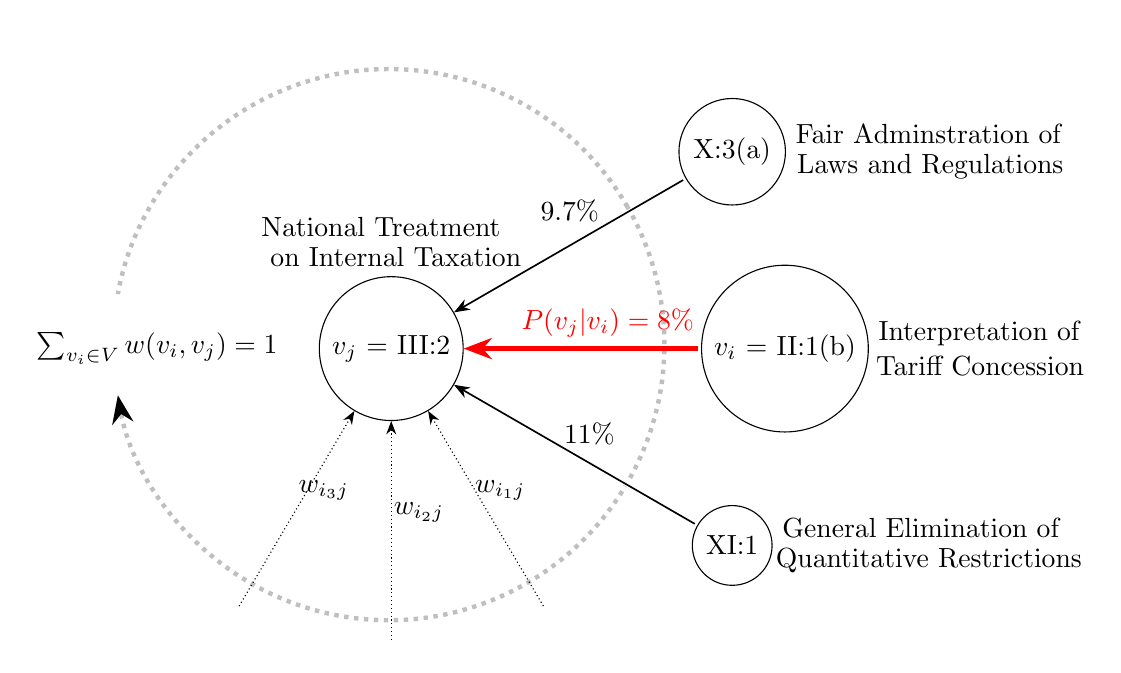
\begin{tikzpicture}[
        >={Stealth[color=black]}
        ,shorten >=1pt,node distance=2cm
        ,on grid,initial/.style={}
        ,every label/.style={align=left}
        ]
        \linespread{2}
        \node[state, label=above:{National Treatment \\[1mm] \hspace{0mm} on Internal Taxation}] (T1) at (10, 0) {$v_j$ = III:2};

        \node[text width=5cm] at (8,0)
        {$\sum_{v_i\in V}{w(v_i, v_j)} = 1$};

        \draw[ultra thick, gray!50, dotted, ->] (13,1.8) arc (30:-170:3.5);
        \draw[ultra thick, gray!50, dotted, -] (13,1.8) arc (30:170:3.5);

        \node[state, label=right:{Interpretation of \\[1mm] \hspace{-1.5mm} Tariff Concession}] at ([shift=({0:5 cm})]T1) (T2) {$v_i$ = II:1(b)};
        \node[state, label=right:{General Elimination of \\[1mm] \hspace{-2mm} Quantitative Restrictions}] at ([shift=({-30:5 cm})]T1) (T3) {XI:1};
        \node[state, label=right:{Fair Adminstration of \\[1mm] \hspace{-1mm} Laws and Regulations}] at ([shift=({30:5 cm})]T1) (T4) {X:3(a)};
        
        \draw[red,arrows={[red]<-}, ultra thick] node[above, xshift=12.75cm] {$P(v_j|v_i) = 8\%$} (T1) -- (T2);

        \begin{scope}[every edge/.append style={<-}] % for directed edge, change "style={->, double=black, draw=white}]"
            \path
            % (T1) edge[red, ultra thick] node[above] {$0.092$} (T2)
            (T1) edge[double=black, draw=white] node[above, xshift=5pt] {$11\%$} (T3)
            (T1) edge[double=black, draw=white] node[above, yshift=5pt] {$9.7\%$} (T4);

            \path[->] (T1) edge[thin,<-,densely dotted] node[above, xshift=5pt] {$w_{i_{1}j}$} +(1.95,-3.3);
            \path[->] (T1) edge[thin,<-,densely dotted] node[above, xshift=10pt] {$w_{i_{2}j}$} +(0,-3.75);
            \path[->] (T1) edge[thin,<-,densely dotted] node[above, xshift=10pt] {$w_{i_{3}j}$} +(-1.95,-3.3);
        \end{scope}

    \end{tikzpicture}

% \begin{figure}[ht]
%     \centering
    
%     \caption{\textbf{Example of Network of Legal Articles of WTO agreements: }}
%     \label{fig:def-example}
% \end{figure}

      }
      \caption{\textbf{Illustration of $P(v_j \mid v_i)$ where the target article $v_j=$ Article III:2}}
      \label{subfig:a:art2b}
  \end{subfigure}
  \vfill
  \begin{subfigure}[b]{1\textwidth}
      \centering{
          \begin{displayquote}[][]
    \begin{center}
    \end{center}
  
    \begin{displayquote}[][]
    ``The dictionary definition of the noun `excess' is `the amount by which one number
        or quantity exceeds another'. More specifically, `in excess of' means `more than'. Thus,
        as a textual matter, a particular number or quantity is `in excess of' another number
        or quantity if it is greater, regardless of the extent to which it is greater. 
      \textbf{\textit{Looking at the context of Article II:1(b), first sentence, we note that Article III:2, first
      sentence, of the GATT 1994 is cast in very similar terms and in fact uses the phrase
      `in excess of'}}:\\
        \begin{displayquote}
        \textit{The products of the territory of any contracting party imported into the
      territory of any other contracting party shall not be subject … to internal
      taxes or other internal charges of any kind in excess of those applied … to
      like domestic products \ldots}
        \end{displayquote}   
    \end{displayquote}  
  \end{displayquote}

      }
      \centering
      \caption{\textbf{Jurisprudence of Panel in \textit{Russia – Tariff Treatment} case:} Panel explains that the meaning of the term \textit{`in excess of'} in Article II:1(b) clarifies the meaning of the same phrase in Article III:2.}
      \label{subfig:a:condprob}
  \end{subfigure}
  \caption{\textbf{Modeling of the Network of Articles of WTO agreements}}
  \label{fig:def-example}
\end{figure}

\section{Modeling and Formal Definitions}
\subsection{Network of Articles of the WTO agreements \label{subsec:def}}

I define the network of articles of WTO agreements as directed weighted graph $G=(V, \vec{E}, W)$ which is comprised of 
vertex set $V$, set of directed edges $\vec{E}$, and edge weight matrix $W$. I define each legal article of WTO agreement as a vertex, thus
$V=\{v \mid v\text{ is a legal article of WTO agreement\}}$. Then I define all ordered pairs of vertices as a set of directed edges $\vec{E}$, thus
$\vec{E} = \{(v_i, v_j) \mid (v_i, v_j)\in V \times V)\}$. 
Finally, I define the edge weight matrix $W=(w(v_i, v_j)) \in [0,1]^{|V| \times |V|}$ where all incoming edge weights sum up to $1$ for all given target vertex $v_j$, thus
$\sum_{v_i\in V}{w(v_i, v_j)}$ = 1. $w$ denotes a map that assigns a weight for each ordered pair of vertices, thus $w : V \times V \to [0,1]$. 
I always assign weight $0$ for the directed edge comprised of the same vertex, thus  $w(v_i, v_i) = 0 \:\: \forall{v_i \in V}$.
For convenience, I define $w_{ij} = w(v_i, v_j)$.


\subsection{Modeling Interaction between Articles of WTO agreements as Conditional Probability}
I interpret every directed edge weight $w(v_i, v_j)$ as the conditional probability $P(v_j|v_i) \in [0,1]$, where the probability represents how probably the source node $v_i$ clarifies the interpretation of the target node $v_j$ comapred to all other source nodes $v\in V \setminus \{v_i, v_{j}\}$. 
The articles of WTO agreements interdependently constitute the legal context to clarify the interpretation of other articles as shown in the the Panel report of \textit{Russia-Tariff Treatment} case, as excerpted in Figure \ref{subfig:a:condprob}. In \textit{Russia-Tariff Treatment} case, the Panel explained that Article II:1(b) clarifies the meaning of the same phrase \textit{`in excess of'} in Article III:2.
By modeling this clarification relationship as the directed edge weight $w_{ij}$, I let the edge weight $w_{ij}$ represent the realtive importance of a source article $v_i$ clarifying the interpretation of the target article $v_j$. I illustrated this relationship in Figure \ref{subfig:a:art2b}.

\subsection{Methodological Objective: Finding $G^*$}
I aim to find $G^* = (V, \vec{E}, W^*)$ where the $W^*$ closely reflect the clarification relationship between articles of WTO agreements as explained by the authoritative judicial bodies of the WTO DSB, Panel and Appellate Body. To find $W^*$, this paper collected the past 20 years of legal dispute data in WTO DSB. The types and composition of the data collected will be explained in Section \ref{sec:data}.
Then I design a deep neural network to encode the pattern of interactions of the articles of WTO agreements found in the data. Justification of using deep learning, design and training of deep neural network, and fitting process of $W^*$ using \textit{Random Forest} will be explained in Section \ref{sec:methods}.
Finally in Section \ref{ef}, I will verify the quality of the fitted $G^*$ by comparing the systematic interaction between articles of WTO agreements found in $G^*$ with the corresponding jurisprudence of the Panel and Appellate Body.

% network $G = (V, \vec{E}, W)$ collect all the relative importance of each article compared to other articles to 

% every directed edge weight $w(v_i, v_j)$ 

% model this clarification relationship as the directed edge weight $w(v_i, v_j)$.

% Above subfigure (a) represents how jurisprudence of \textit{Panel} stated in (b) is represented as an edge weight where the source node Article II:1(b) constitutes the legal context of the target node Article III:2 regarding how to interpret its term \textit{`in excess of'} with the $8\%$ of importance compared to other possible source articles.}

% The system has become more complex as the number of cases requested to WTO DSB increases and developing countries can't resolve their dissatisfaction over the trade relationship in WTO DSB.

% Moreover, I aim to summarize the network of WTO articles as a whole not by parts.
% There already exists numerous literatures that studied the relationship between articles of WTO agreements \citep{chadXXIII, charnovitz, Trachtman, who_gets}.
% However, previous literatures have been limited to studying the interconnections between relatively small number of articles, which are mostly less than 10. % and has not been conducted in a level of entire WTO agreements. As my method captures the entire systematic correlation between the articles of WTO agreements, it becomes 
% By pursuing a holistic approach, I intend to enhance the practicalness of the method. The legal system of WTO always works as whole and the entire system provide legal contexts to its sub-systems \citep{system_as_a_whole}.

% In other words, this method effectively materializes the shared understanding of legal experts thus can lower the cost to build the same amount of legal capacity to understand the WTO DSB.
% Moreover, rather than keep relying on previous approach that provides legal advice to developing countries that does not create a shared understanding over the system between developing and developed countries,
% if we shift our focus on how to materialize the current shape of the system, WTO
% will become more effective as members being able to discuss their trade issues upon the measurable ground of shared understanding about how WTO works.




% way of the fitted network $G^*$ explaining how articles of WTO agreements achieve some main principles of WTO, such as \textit{Market Access}, \textit{Reciprocity} and \textit{Non-discrimination}



% fitted a set of directed edge weights $W^*$ that
% best explains the variance of each article's citabilities that are predicted by the trained deep neural network using a machine learning technique \textit{Random Forests} \citep{rf, genie3}.
 
% After fitting $W^*$, to check whether this fitted network of articles of the WTO agreements\\  $G^*$ = ($V$, $E$, $W^*$) maps the jurisprudences of WTO DSB properly, this paper
% compares the way of the fitted network $G^*$ explaining how articles of WTO agreements achieve some main principles of WTO, such as \textit{Market Access}, \textit{Reciprocity} and \textit{Non-discrimination}
% with the jurisprudences of \textit{Panel} and \textit{Appellate Body}. This comparison reveals that the fitted network $G^*$ captures the interactions between the articles of WTO agreements
% closely to the jurisprudences of \textit{Panel} and \textit{the Appellate Body}. We can infer from this similarity that the fitted network $G^*$ closely maps the jurisprudences of WTO DSB. This is because those two judicial bodies
% authoritatively constitute the jurisprudences over how rules of WTO agreements are working together
% to achieve those main principles.
 
% Finally, upon this similarity, this paper offers this methodology as
% an alternative solution to the widening gap of legal capacity between developing and developed countries in WTO DSB.
% Since this method effectively materializes the shared understanding of legal experts and reveals important interactions between articles inside the system of WTO DSB,
% it can lower the cost to build the same amount of legal capacity to understand the WTO DSB.
% Moreover, rather than keep relying on previous approach that provides legal advice to developing countries that does not create a shared understanding over the system between developing and developed countries,
% if we shift our focus on how to materialize the current shape of the system, WTO
% will become more effective as members being able to discuss their trade issues upon the measurable ground of shared understanding about how WTO works.
 



% Therefore, this paper designs a deep neural network (\textit{See} Figure \ref{fig:design-of-nn} and \ref{fig:dnn-flow}) that
% processes two different types of textual information.
% One is textual description of the dispute (\textit{See} an example at \hyperref[sub:factual-aspect-example]{Appendix A.1}) and
% the other one is the text of a legal article of the WTO agreements (\textit{See} an example at Figure \ref{fig:gatt_art1}).
% This design is improvised to mimic
% the reasoning process of WTO legal practitioners
% where the legal practitioners read
% the textual description of
% factual circumstances of the dispute and imagine applicable regulatory contents of
% the legal articles while he/she reads that factual description of the case (\textit{See} Figure \ref{fig:viz:how-member-cites-citable}, \ref{fig:viz:how-member-cites-non-citable} and \ref{fig:design-of-nn}).


% The legal system of WTO is understood as a complex network of articles of WTO agreements.
% The articles of WTO agreements interact with each other to constitute specific norms and regulates specific trade issues.
% There exists a numerous literatures that studies the relationship between articles of WTO agreements \citep{chadXXIII, charnovitz, Trachtman, who_gets}.
% However, previous literatures have been limited to study the interconnection between relatively small number of articles, which are mostly less than ten. % and has not been conducted in a level of entire WTO agreements.
% Since the legal system of WTO comprises 


% To address this issue, I provide a novel method to summarize the network of WTO articles as a whole.




% aims to find out the network of legal articles of WTO agreements as a whole.

% This kind of research that studies the relationship between articles of WTO agreements has been actively pursued in numerous literatures \citep{chadXXIII, charnovitz, Trachtman, who_gets}, however, those efforts has been limited to


% The entire map of this network between articles of WTO agreements has been exclusively shared among a group of legal experts of the WTO agreements.



% network of interconnection between articles of WTO agreements is exclusively shared among a group of legal experts of the WTO agreements. 
% This exclusiveness becomes more severe as the number of cases requested to WTO DSB increases and this has led to a widening gap of legal capacities between developing and developed countries.
% This gap now inhibits the effectiveness of the WTO because developing countries are excluded from the WTO DSB to resolve their dissatisfaction over the trade relationship with other members.
% The legal system of WTO is understood as a complex network of articles of WTO agreements.




% This process requires enormous legal knowledge and resources.


% A trade dispute tend to involve complex issue structure.


% because it requires many legal experts to structure a legal argument with a full understanding of the WTO legal system.


% and 

% The legal system of WTO is understood as a complex network of articles of WTO agreements.
% Each part of the network constitutes specific norms and regulates specific trade issues.




% where each part of network handles each 


% between articles are constituting specific norms and regulating specific trade issues.


% Countries usually cite multiple articles to claim their impaired benefits in WTO DSB.

% and the legal system of WTO DSB has evolved into complex network of articles where the interconnectedness between articles are constituting specific norms and regulating specific trade issues.

% This process requires enormous legal knowledge and resources because a trade dispute tend to involve several interconnected trade issues.

% to handle those trade disputes.

% analyzing the network of articles of the WTO agreements provides us a clear view on how WTO DSB constitutes specific norms and regulates specific trade issues.


% Therefore, countries tend to cite multiple articles of WTO agreements to claim their impaired benefits in WTO DSB.

% % Citation of articles of the WTO agreements are evidence of how WTO rules are applied in the real world.


% Therefore, a lawsuit tends to cite multiple rules of the WTO agreement because one simple rule can't cover the complex characteristics of the trade policy that led to the dispute \citep{palmeter2004dispute}.
% For example, the United States enacted \textit{Continued Dumping and Subsidy Act of 2000} (CDSOA) that distributes
% the collected anti-dumping duties to its affected domestic producers.
% This act was challenged by other members with several rules of
% the WTO agreements such as \textit{rules of anti-dumping} and \textit{rules of subsidy}. This was because
% this distribution could constitute an illegal subsidy and illegal anti-dumping duty at the same time as stated in the Panel report of the \textit{US - Offset (CDSOA)} case%(\textit{See} Figure \ref{fig:complex-measure}).

% \blockquote{
%   8.1 In the light of our findings, we conclude that \textbf{the CDSOA is inconsistent with AD (Anti-dumping)
%   Articles 5.4, 18.1 and 18.4, SCM (Subsidy and Countervailing Measure) Articles 11.4, 32.1 and 32.5,} Articles VI:2 and VI:3 of the GATT
%   1994, and Article XVI:4 of the WTO Agreement. \ldots\\
%   8.3 \textbf{The CDSOA is a new and complex measure, applied in a complex legal environment}. In
%   concluding that the CDSOA is in violation of the above mentioned provisions, we have been
%   confronted by sensitive issues regarding the use of subsidies as trade remedies.
%   this matter through negotiation.
% }

% % Citation of articles of the WTO agreements are evidence of how WTO rules are applied in the real world.
% Since multiple articles cooperate to deal with the real world dispute, analyzing the network of articles of the WTO agreements provides us a clear view on how WTO DSB constitutes specific norms and regulates specific trade issues.
% % Principle of \textit{Market Access} which is one of the most important principles in WTO is achieved through a cooperation of multiple articles of the WTO agreements %(Figure \ref{fig:market-aceess_directed}) 
% % and those cooperation is realized through the act of citation by members.
% % Therefore, analyzing the network of articles of the WTO agreements provides us a clear view on how WTO DSB constitutes specific norms and regulates specific trade issues.
% This kind of research that studies the relationship between articles of WTO agreements has been actively pursued in numerous literatures \citep{chadXXIII, charnovitz, Trachtman, who_gets}, however, those efforts has been limited to
% study interconnectedness between relatively small numbers (less than 10) of articles. % and has not been conducted in a level of entire WTO agreements.

% Therefore, this research aims to find out the network of legal articles of WTO agreements as a whole.
% Currently, the entire map of interconnection between articles of WTO agreements is exclusively shared among a group of legal experts of the WTO agreements.
% This exclusiveness becomes more severe as the number of cases requested to WTO DSB increases and this has led to a widening gap of legal capacity between developing and developed countries.
% This gap now inhibits the effectiveness of the WTO because developing countries are excluded from the WTO DSB to resolve their dissatisfaction over the trade relationship with other members.
% % at this moment and members are discussing possible solutions under the agenda of \textit{WTO reform}
% % but proposed solutions are mainly about unilateral support of legal resources from the developed countries to developing countries and this solution has been ineffectiveness reflecting on the similar efforts during the past decades of WTO DSB.
% % such as principle of \textit{Market Acceess} (across borders),
% % \textit{Non-discrimination} (between members
% % or between domestic products and imported products)
% % and \textit{Transparency} (in publication and maintaining
% % of each member's internal regulations),
% % it's intellectually intriguing
% % to understand how regulatory system of WTO DSB
% % is structured to achieve these main principles (\textit{See} Figure \ref{fig:market-aceess_directed}).
% % By understanding this structure,
% % we can improve WTO system to serve its main prinicples more effectively
% % and to adopt to constantly
% % changing world trade circumstances
% % \citep{FREDEBEULKREIN1999625, shaffer_2004, 10.1093/jiel/jgm028}.
% % Therefore, this paper emphasizes the importance of revolutionizing the way of studying network of articles of WTO agreements 

% Therefore, this paper provides a novel method to summarize the network of articles of WTO agreements. 
% % This network materializes the relationship between the articles of the WTO agreements as a .
% This paper maps
% the jurisprudence of WTO DSB
% as a network of legal articles
% as formally defined as

% in Figure \ref{fig:def} and illustrated in Figure \ref{fig:def-example}. This is because the rules of the WTO agreements
% explicitly requires \textit{Panel} or \textit{Appellate Body} to address
% relevant articles together when they construct its jurisprudence related to the meaning, scope and interpretation of any legal text in the WTO agreements as excerpted in Figure \ref{fig:art7dsu}.
% Upon this requirement, judicial bodies cite
% multiple articles together
% to identify the complex legal identity of a trade policy at issue as clearly opinionated in Figure \ref{fig:complex-measure}.
% In addition to it, judicial bodies cite multiple articles together
% to guide an way of interpretation of the rules of the WTO agreements (\textit{See} Figure \ref{subfig:a:condprob}).
% % \begin{figure}[h]
% %   \begin{quote}
% %       8.1 In the light of our findings, we conclude that \textbf{the CDSOA is inconsistent with AD (Anti-dumping)
% %       Articles 5.4, 18.1 and 18.4, SCM (Subsidy and Countervailing Measure) Articles 11.4, 32.1 and 32.5,} Articles VI:2 and VI:3 of the GATT
% %       1994, and Article XVI:4 of the WTO Agreement. \ldots
% %   \end{quote}
% %   % \begin{quote}
% %   %     \centering{\ldots}
% %   % \end{quote}
% %   \begin{quote}
% %       8.3 \textbf{The CDSOA is a new and complex measure, applied in a complex legal environment}. In
% %       concluding that the CDSOA is in violation of the above mentioned provisions, we have been
% %       confronted by sensitive issues regarding the use of subsidies as trade remedies.
% %       this matter through negotiation.
% %   \end{quote}
% %   \caption{\textbf{Panel's Judicial Opinion On the \textit{US - Offset (Byrd Amendment; CDSOA)} case:} Panel explicitly expresses the complexity of the trade policy (CDSOA) at issue and cites the rules of anti-dumping (AD) and subsidy (SCM) at the same time to cover its complex characteristics.}
% %   \label{fig:complex-measure}
% % \end{figure}
% To develop a proper method that can find a set of directed edge weights $W$ defined in Figure \ref{fig:def}
% as close to a shared understanding of legal experts, this paper points out two main considerations.
% First, one need to use information inside a textual description of factual circumstances of the legal dispute and the regulatory contents inside the text of each article of the WTO agreements.
% Second, one need to generalize the members' strategic citation pattern that is limited to a member-specific political interest.
% For example, members strategically cite different rules of the WTO agreements to limit or to encourage
% the third party participation. Since the third party participation
% can lead to early settlement of the dispute without continuous
% legal battle, members cite differently according to their intention to
% settle the case earlier out of court \citep{who_gets}. Moreover, members cite articles strategically trying to reshape the legal precedents of WTO DSB
% in favor of their future interest \citep{pelc, latent}.
% % For example,
% % members tend to cite their
% % favorable previous cases more often in issue areas where they face ligitagion more frequently with other members
% % \citep{latent}.
% Upon these two considerations, this paper selects the deep neural network as a technical solution. % to effectively extract information from the text and to generalize the member specific strategic citation patterns.
% This is because a deep neural network is empirically known as good at extracting information from text and generalizing the patterns inside data.
% Therefore, this paper designs a deep neural network (\textit{See} Figure \ref{fig:design-of-nn} and \ref{fig:dnn-flow}) that
% processes two different types of textual information.
% One is textual description of the dispute (\textit{See} an example at \hyperref[sub:factual-aspect-example]{Appendix A.1}) and
% the other one is the text of a legal article of the WTO agreements (\textit{See} an example at Figure \ref{fig:gatt_art1}).
% This design is improvised to mimic
% the reasoning process of WTO legal practitioners
% where the legal practitioners read
% the textual description of
% factual circumstances of the dispute and imagine applicable regulatory contents of
% the legal articles while he/she reads that factual description of the case (\textit{See} Figure \ref{fig:viz:how-member-cites-citable}, \ref{fig:viz:how-member-cites-non-citable} and \ref{fig:design-of-nn}).
% % As WTO sets its main principles to regulate the world trade system in general
% % such as principle of \textit{Market Access} (across borders),
% % \textit{Non-discrimination} (between members
% % or between domestic products and imported products)
% % and \textit{Transparency} (in publication and maintaining
% % of each member's internal regulations),
% % it's intellectually intriguing
% % to understand how regulatory system of WTO DSB
% % is structured to achieve these main principles (\textit{See} Figure \ref{fig:market-aceess_directed}).
% % By understanding this structure,
% % we can improve WTO system to serve its main principles more effectively
% % and to adopt to constantly
% % changing world trade circumstances
% % \citep{FREDEBEULKREIN1999625, shaffer_2004, 10.1093/jiel/jgm028}.
% % Moreover, members' citation of articles of the WTO agreements also gets complicated
% % if we consider the fact that \textit{Panel} or \textit{Appellate Body} defers to the legal precedents of WTO DSB.
% % Legal precedents refer to \textit{Panel} or \textit{Appellate Body}'s judicial decisions
% % and these legal precedents provide authoritative reference
% % for deciding subsequent cases in WTO DSB.
% % Members try to reshape these legal precedents
% % in favor of their future interest more than
% % simply using the WTO DSB to resolve their trade
% % dispute \citep{pelc}. For example,
% % members tend to cite their
% % favorable previous cases more often in issue areas where they face ligitagion more frequently with other members
% % \citep{latent}.
% % as close to
% % a shared understanding of legal experts of the WTO agreements, one needs to understand how members cites articles of the WTO agreements in WTO DSB.
% % However, Citation of the rules of the WTO agreements tends to get more complicated because members cite the
% % rules of the WTO agreements strategically.
% % \footnote{
% % \blockquote{
% %     The CDSOA is a new and complex measure, applied in a complex legal environment. In
% % concluding that the CDSOA is in violation of the above mentioned provisions, we have been
% % confronted by sensitive issues regarding the use of subsidies as trade remedies. If Members are of the
% % view that subsidisation is a permitted response to unfair trade practices, we suggest that they clarify
% % this matter through negotiation
% % }
% % }
 
 
 


Moreover, legal citation becomes even more complicated because members cite the 
rules of the WTO agreement strategically. For example,
members cite different rules of the WTO agreement to limit or to encourage 
the third party participation because the third party 
participation can lead to eary settlement of the dispute without continuos 
legal battle and vice versa  \cite{who_gets}.
% As WTO sets its main principles to regulate the world trade system in general
% such as principle of \textit{Market Acceess} (across borders), 
% \textit{Non-discrimination} (between members 
% or between domestic products and imported products) 
% and \textit{Transparency} (in publication and maintaining 
% of each member's internal regulations), 
% it's intellectually intriguing 
% to understand how regulatory system of WTO DSB
% is structured to achieve these main principles (\textit{See} Figure \ref{fig:market-aceess_directed}).
% By understanding this structure, 
% we can improve WTO system to serve its main prinicples more effectively 
% and to adopt to constantly
% changing world trade circumstances
% \citep{FREDEBEULKREIN1999625, shaffer_2004, 10.1093/jiel/jgm028}.


However, it is extremely difficult to map how regulatory network of 
WTO DSB is organized to acheive the core principles of WTO. 
This is because 
each citation is closely related 
to the composite characteristics of each trade policy 
as explained in the above example, \textit{Byrd Amendment}. 
Moreover, one needs to generalize the above mentioned strategic 
citation in WTO DSB which is limited to each member's 
specific political interest rather than explaining the 
regulatory power of WTO DSB in general. 


To address this issue, 
this paper maps 
the regulatory system of WTO DSB 
as a network of legal articles 
of the WTO agreements as exemplified in the Figure \ref{fig:market-aceess_directed} 
and formally defined in Figure \ref{fig:def}. This is because rules of the WTO agreements
% \footnote{\textit{See} Article 7 in Dispute Settlement Rules: Understanding on Rules and Procedures Governing the Settlement of Disputes, Marrakesh Agreement Establishing the World Trade Organization, Annex 2, 1869 U.N.T.S. 401, 33 I.L.M. 1226 (1994)} 
explicitly requires judicial bodies to address 
relevant articles together to construct its jurisprudence (Figure \ref{fig:art7dsu}).
Upon this requirement, judicial bodies refer to 
multiple articles of the WTO agreements together
to identify the complex legal identity of the trade policy that led to the dispute.
In addition to it, judicial bodies cite multiple articles together 
to provide an authoritative interpretation of the rules of the WTO agreements
\citep{oesch2003standards}.

\begin{figure}
  \begin{displayquote}[][]
    \begin{center}
      Article 7
    \end{center}
    \begin{center}
      Terms of Reference of Panels
    \end{center}
  
    1. Panels shall have the following terms of reference unless the parties to the dispute
    agree otherwise within 20 days from the establishment of the panel:
  
    \begin{displayquote}[][]
  
      ``To examine, in the light of {\bf the relevant provisions} in (name of the covered
      agreement(s) cited by the parties to the dispute), the matter referred to the DSB by
      (name of party) in document … and to make such findings as will assist the DSB in
      making the recommendations or in giving the rulings provided for in that/those
      agreement(s).''
        
    \end{displayquote}
  
    2. Panels shall address {\bf the relevant provisions} in any covered agreement or agreements
    cited by the parties to the dispute. \ldots
  \end{displayquote}
  \caption{\textbf{Article 7 of the Dispute Settlement Understanding (DSU): } 
  DSU provides a legal guidelines on how judicial boides of WTO shall adjudicate the requested disputes.
  It explictly requires judicial bodies to interweave relevant articles of the WTO agreements to clarify
  it's meaning, scope and interpretation.
  } 
  \label{fig:art7dsu}
\end{figure}



\begin{figure}[ht]
\[\text{Network of legal articles of WTO agreement is defined as }  G = (V, E, w) \] 
\[\text{ where } V = \{v \mid v\text{ is a legal article of WTO agreement}\}  \text{ , } \]
\[\vec{E} = \{(v_1, v_2) \mid (v_1, v_2)\in V \times V)\} \text{ and }w : V \times V \to \Bbb R_{+} \]
\[G\text{ is simply called \textit{directed weighted graph}}\]
\caption{\textbf{Formal Definition of Network of Legal Articles of WTO agreements}}
\label{fig:def}
\end{figure}

% \begin{displayquote}
%     \center{Article 7}

%     \center{Terms of Reference of Panels}

%     1. Panels shall have the following terms of reference unless the parties to the dispute
%     agree otherwise within 20 days from the establishment of the panel:
%     "To examine, in the light of the relevant provisions in (name of the covered
%     agreement(s) cited by the parties to the dispute), the matter referred to the DSB by
%     (name of party) in document … and to make such findings as will assist the DSB in
%     making the recommendations or in giving the rulings provided for in that/those
%     agreement(s)."
%     2. Panels shall address the relevant provisions in any covered agreement or agreements
%     cited by the parties to the dispute.
% \end{displayquote}


To train this neural network, this paper collected textual description of trade policy 
that led to the dispute and articles of the WTO agreement cited for each dispute
case requested to the WTO DSB 
from 1995 to 2018 (\hyperref[sub:cited-articles-table]{Total $143$ cases. \textit{Check} the list in Appendix A.2}).
Using this collected data, I trained the neural network by enforcing the neural network to answer correctly 
whether a given article of the WTO agreements
can be cited for the given textual description of 
trade policy. (\textit{See} Figure \ref{fig:design-of-nn} and Figure \ref{fig:def:io:nn}).

After training, I fitted a set of directed edge weights $W^*$ that 
best explains the variance of each article's citabilities that are predicted by the trained deep neural network using a machine learning technique \textit{Random Forests} \citep{rf, genie3}. 

After fitting $W^*$, to check whether this fitted network of articles of the WTO agreements\\  $G^*$ = ($V$, $E$, $W^*$) maps the jurisprudences of WTO DSB properly, this paper
compares the way of the fitted network $G^*$ explaining how articles of WTO agreements achieve some main principles of WTO, such as \textit{Market Access}, \textit{Reciprocity} and \textit{Non-discrimination} 
with the jurisprudences of \textit{Panel} and \textit{Appellate Body}. This comparison reveals that the fitted network $G^*$ captures the interactions between the articles of WTO agreements
closely to the jurisprudences of \textit{Panel} and \textit{the Appellate Body}. We can infer from this similarity that the fitted network $G^*$ closely maps the jurisprudences of WTO DSB. This is because those two judicial bodies 
authoritatively consitute the jurisprudences over how rules of WTO agreements are working together 
to achieve those main principles.

Finally, upon this similarity, this paper offers this methodology as
an alternative solution to the widening gap of legal capacity between developing and developed countries in WTO DSB.
Since this method effectively materializes the shared understanding of legal experts and reveals important interactions between articles inside the system of WTO DSB,
it can lower the cost to build the same amount of legal capacity to understand the WTO DSB.
Moreover, rather than keep relying on previous approach that provides legal advice to developing countries that does not create a shared understanding over the system between developing and developed countries,
if we shift our focus on how to materialize the current shape of the system, WTO
will become more effective as members being able to discuss their trade issues upon the measurable ground of shared understanding about how WTO works.


% \begin{itemize}
%     \item It shows that the result neural network well match with the result of main two judicial bodies.
% \end{itemize}



\section{Data}
I collected two different types of data for 143 dispute cases 
requested to the WTO DSB.
One is textual description of trade policy 
that led to the dispute \hyperref[sub:factual-aspect-example]{(Appendix A.2)} and the other one is 
set of articles of the WTO agreement that are
cited for each dispute. 
I will explain the format and the content of 
each type of data with an example. 
Technical details about the automated way 
of collecting and cleansing the data is 
explained in the \hyperref[sec:appendix]{Appendix}.


% This section explains how I collected 
% which data to train the neural network. 
% Basically, 





% I collected two different 
% types of data, one is textual description of trade policy 
% that led to the dispute and the other one is 
% set of articles of the WTO agreement that are
% cited for the dispute.s



% \begin{displayquote}
%     ``Korea' s domestic support for beef in 1997 and 1998 exceeded the de minimis level contrary to Article 6 of the Agreement on Agriculture.''
%   \end{displayquote}
  
%   \begin{itemize}
%     \item exemplify as detail as possible to inform readers about how data looks like.
%     \item Privide a running example that shows how WTO works with data. 
%     \item (Borrow from the previous paper)
    
%   \end{itemize}
  

% \subsection{General Explain}
% \begin{itemize}
    \item How WTO works with its typical rhetorics - "inconsitent with" .. with example
\end{itemize}

\subsection{Factual Aspect}
Textual description of the dispute is preferably called as
\textit{Factual Aspect} in WTO DSB.
Since Panel
always provide a factual aspect\footnote{
  It's worth noting that Appellate Body doesn't provide any factual aspect because they always use the factual aspect provided by the Panel.
}
that describes the circumstances of the dispute
in each report, %(Figure \ref{fig:panel-report-toc}),
I wrote a program that
automatically search and collect
the panel reports from the WTO official document website\footnote{
  \url{http://docs.wto.org}
}.
Then I located the factual aspect using the page information from the
table of contents in each panel report as shown in Figure \ref{fig:panel-report-toc}.
I collected the total 143 numbers of different factual aspects . The collected case numbers are listed in Figure \ref{fig:ds-cases-used}.

\subsubsection{Joint Adjudication \& Early Settlement}
The number 143 may seem small compared to the total 596\footnote
{As of November 1st, 2020.} number of cases that are requested to WTO DSB. This is due to the following two reasons.
First, panel jointly adjudicates different cases together if the cases raise the claim toward the
same trade policy of the same member state. For example, in \textit{US - Offset (Byrd Amendment)}, panel merged DS217\footnote{
  DS refers to \textit{Dispute Settelement}. DS is the official prefix that indicates the case in WTO DSB.
} and DS234 together because they were asking the judicial opinion for the same government measure of the United States as shown in Figure \ref{fig:linked-cases}.
This paper selects the smallest case number as a representative number for this case of joint adjudication.
For example, DS217 and DS234 share the same panel report then this paper chooses DS217 as a representative number as shown in Figure \ref{fig:ds-cases-used} where the list includes DS217 but not DS234.
Second, members sometimes find \textit{mutually agreeable solution} before the panel expresses its judicial opinion by publishing its panel report. Then Panel stops there and no factual aspect is provided. I omitted this kind of \textit{early settled} cases as well.
% \subsubsection{Judicial Economy \& Early Settlement}
\begin{figure}[t!]
  \begin{quote}
      DS 2,
      18,
      22,
      31,
      34,
      46,
      56,
      58,
      60,
      62,
      67,
      68,
      69,
      75,
      76,
      87,
      90,
      98,
      103,
      108,
      121,
      122,
      135,
      136,
      139,
      141,
      146,
      152,
      155,
      161,
      162,
      165,
      166,
      174,
      175,
      177,
      184,
      202,
      207,
      212,
      217,
      219,
      221,
      231,
      234,
      238,
      244,
      245,
      246,
      248,
      257,
      264,
      265,
      266,
      267,
      268,
      269,
      276,
      282,
      283,
      286,
      290,
      294,
      295,
      296,
      301,
      302,
      308,
      312,
      315,
      316,
      320,
      321,
      322,
      332,
      336,
      339,
      343,
      344,
      345,
      350,
      353,
      360,
      363,
      366,
      371,
      379,
      381,
      384,
      392,
      394,
      396,
      397,
      399,
      400,
      406,
      412,
      414,
      415,
      422,
      425,
      427,
      429,
      430,
      431,
      435,
      436,
      437,
      440,
      442,
      447,
      449,
      453,
      454,
      456,
      457,
      461,
      464,
      468,
      471,
      472,
      473,
      475,
      476,
      477,
      479,
      480,
      482,
      483,
      484,
      485,
      486,
      488,
      490,
      492,
      493,
      495,
      499,
      504,
      505,
      513,
      518,
      523
  \end{quote}
  \caption{
      \textbf{List of the Collected Case numbers:} ``DS + number'' uniquely identifies each dispute. For example, DS 523 refers to \textit{US — Pipe and Tube Products (Turkey)} where the United States was challenged by Turkey for its possibly inconsistent anti-dumping measure.
      % where Turkey claimed claimed possible illegal trade policy of United States on pipe ane tube products from Turk.
  }
  \label{fig:ds-cases-used}
\end{figure}
\begin{figure}[t!]
  \centering
  \frame{
    \includegraphics[scale=0.35]{Data/pngs/linked_cases.png}
  }
  \caption{\textbf{Cover of a Panel Report Includes Information about Joint Adjudication:}
      Panel explicitly marks which different cases are adjudicated together in the cover of the panel report. DS217 and DS234 are handled together in this example.
      }
  \label{fig:linked-cases}
\end{figure}
% way before they express their
% legal conclusion as to the inconsistency  to the rules of the WTO or not.
% where the panel expresses
% its conclusion as to whether the challenged
% trade policy is inconsistent to the rules of the WTO or not.
 
 
 



\subsection{Cited Articles}
Every lawsuit in WTO DSB 
has its own set of aritcles cited by complainant(s)
as shown in Table 
\ref{xltabular:cited-article-for-us-offset}. 
I wrote a program that collects a set of articles cited for 
each case from WTO official webpage\footnote{\url{https://www.wto.org/english/tratop_e/dispu_e/dispu_status_e.htm}}. 
The webpage chronologically lists up all dispute cases
requested to WTO DSB and the prgoram visits each dispute page of 143 cases
and collects cited articles for each case. Among all the articles from different agreements
of the WTO agreements\footnote{
    WTO agreeemnts is comprised of mutiple agreements such as
    General Agreement on Tariffs and Trade 1994,
    Agreement on Agriculture,
    Agreement on the Application of Sanitary and Phytosanitary Measures,
    Agreement on Textiles and Clothing,
    Agreement on Technical Barriers to Trade,
    Agreement on Trade-Related Investment Measures,
    Agreement on Implementation of Article VI of the General Agreement on Tariffs and Trade 1994 (antidumping),
    Agreement on Subsidies and Countervailing Measures,
    Agreement on Rules of Origin,
    Agreement on Safeguards and so on.
    } ,
this paper collected articles from General Agreement on Tariffs and Trade 1994 (GATT 1994) only. 
This is because articles in GATT 1994 constitutes basic set of trade rules of WTO and other agreements 
elaborates the articles of GATT 1994 more in detail \citep{world1999wto}. For example, the official name of \textit{Agreement on Anti-dumping}
is \textit{Agreement on Implementation of Article VI of the General Agreement on Tariffs and Trade 1994}
where the name itself explians its relationship to GATT 1994.
The collected result is listed in the \hyperref[sub:cited-articles-table]{Appendix A.2} and Figure \ref{fig:set-of-articles-used} 
lists distinct 80 articles of GATT 1994 cited in 143 cases without duplication. 

\begin{figure}[h]
    \begin{quote}
    I, 
    I:1, 
    II, 
    II:1, 
    II:1(a), 
    II:1(b), 
    II:2, 
    II:3, 
    III, 
    III:1, 
    III:2, 
    III:4, 
    III:5, 
    III:7, 
    IV, 
    IX, 
    IX:2, 
    V, 
    V:1, 
    V:2, 
    V:3, 
    V:3(a), 
    V:4, 
    V:5, 
    V:6, 
    V:7, 
    VI, 
    VI:1, 
    VI:2, 
    VI:2(a), 
    VI:2(b), 
    VI:3, 
    VI:5(a), 
    VI:6, 
    VII, 
    VII:1, 
    VII:2, 
    VII:5, 
    VIII, 
    VIII:1, 
    VIII:3, 
    VIII:4, 
    X, 
    X:1, 
    X:2, 
    X:3, 
    X:3(a), 
    XI, 
    XI:1, 
    XIII, 
    XIII:1, 
    XIII:2, 
    XIII:3(b), 
    XIX, 
    XIX:1, 
    XIX:2, 
    XIX:3, 
    XV, 
    XVI, 
    XVI:1, 
    XVI:4, 
    XVII, 
    XVII:1, 
    XVII:1(c), 
    XVIII, 
    XVIII:10, 
    XVIII:11, 
    XX, 
    XXI, 
    XXII, 
    XXII:1, 
    XXIII, 
    XXIII:1, 
    XXIII:1(a), 
    XXIII:1(b), 
    XXIV, 
    XXIV:12, 
    XXIV:5(b), 
    XXIV:6, 
    XXVIII
    \end{quote}
    \caption{Set of articles of GATT 1994 used in this paper}
    \label{fig:set-of-articles-used}
\end{figure}

\subsubsection{Various Levels of Scope in Cited Articles}
As shown in Figure \ref{fig:set-of-articles-used}, 
members sometimes
cite articles in different levels of scope. For example, 
For the Article VI, member sometimes cites
Article VI as a whole but sometimes cites
Article VI:2 or Article VI:2(a).
This is because two main judicial bodies of WTO DSB, Panel and Appellate Body, 
both constitutes its jurisprudence using
various level of scope to interpret the legal texts of the WTO agreements,
such as in the level of \textit{Title, Article, Paragraph, Sentence or Term} as shown in Table {\ref{xltabular:level-of-scopes}}. 
Following this jurisprudence, members also cite articles in different levels of scope to 
make their legal claim valid as much as possible.

\begin{xltabular}{\linewidth}{lXX}
    \hline
    \textbf{\normalsize Scope} 
    & \textbf{\normalsize Quote}
    & \textbf{\normalsize Source}
    \\
    \endfirsthead
    \hline \hline \hline


    Title
    & ``As the \textbf{\textit{title}
    of Article 21 makes clear}, 
    the task of panels \ldots
    forms part of the process
    of the `Surveillance of 
    Implementation of the 
    Recommendations and Rulings' of the
    DSB. \ldots'' 
    & Appellate Body Report, \textit{US – Shrimp (Malaysia)}, paras. 86-87.
    \\
    \hline
    Article 
    &  ``The sequence of steps indicated above in the analysis of a claim of justification under \textbf{Article XX} reflects, not inadvertence or random choice, but rather the fundamental structure and logic of Article XX. \ldots''
    & Appellate Body Report, \textit{US – Shrimp (Malaysia)}, paras. 119-120.
    \\
    \hline
    Paragraph
    &  ``The verb 'may' in \textbf{Article VI:2} of the GATT 1994 is, in our opinion, properly
    understood as giving Members a choice between imposing an anti-dumping duty or
    not, as well as a choice between imposing an anti-dumping duty equal to the dumping
    margin or imposing a lower duty. \ldots''
    & Appellate Body Report, \textit{US – 1916 Act}, paras. 116.     
    \\
    \hline
    Sentence 
    & ``The customary rules of interpretation of public international law as
    required by \textbf{the first sentence of Article 17.6(ii) of the Anti-Dumping Agreement}, do
    not admit of another interpretation as far as the issue of zeroing raised in this appeal
    is concerned.''
    & Appellate Body Report, \textit{US – Zeroing (EC)}, paras. 132-133.
    % \hline
    % \textbf{\normalsize Scope} 
    % & \textbf{\normalsize Quote}
    % & \textbf{\normalsize Source}
    \\
    \hline
    Term
    & ``Article II:1(a) provides that a
    Member shall accord to the `commerce' of other Members treatment no less
    favourable than that provided for in its Schedule. \textbf{The term `commerce'} is defined as
    referring broadly to the exchange of goods such that, in this provision, the 'commerce'
    of a Member should be understood to refer to all such exchanges of that Member''
    & Appellate Body Report, \textit{Colombia – Textiles}, para. 5.34.
    \\
    \hline
    \caption{Various levels of scope appearing in the jurisprudence of WTO DSB}
    \label{xltabular:level-of-scopes}

\end{xltabular}


% \begin{figure}[h]
% \begin{quote}
%     \ldots As the \textit{title} of Article 21 makes clear, the task of panels \ldots
%      forms part of the process
%     of the 'Surveillance of Implementation of the Recommendations and Rulings' of the
%     DSB. - \textit{Appellate Body Report, US – Shrimp (Malaysia), paras. 86-87. }
% \end{quote}
% \caption{Various Interpretative Scopes of Panel and Appellate Body}
% \end{figure}

% paragraph is also important in terms of scope.



\section{Methodology}
\subsection{Limits of Naive Approach}

\begin{itemize}
  \item Compare co-occurrences/neural network approach.

  \item Show that co-occurrences approach isn't accurate.
\end{itemize}


\section{Empirical Findings}

\begin{itemize}
  \item No Greeks. English. Three Networks.
\end{itemize}

% == THREE SUBSYSTEM == 
\begin{figure}[ht]
    \centering{
      % 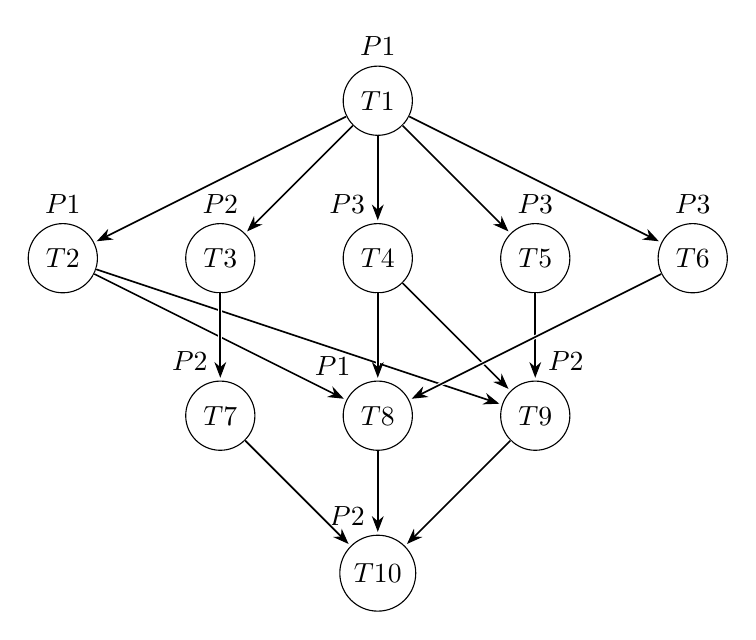
\begin{tikzpicture}[>={Stealth[color=black]},shorten >=1pt,node distance=2cm,on grid,initial/.style={}]
        \node[state, label=above:$P1$] (T1) {$T1$};
        \node[state, label=95:$P3$] (T4) [below =of T1] {$T4$};
        \node[state, label=above:$P2$] (T3) [left  =of T4] {$T3$};
        \node[state, label=above:$P1$] (T2) [left  =of T3] {$T2$};
        \node[state, label=above:$P3$] (T5) [right =of T4] {$T5$};
        \node[state, label=above:$P3$] (T6) [right =of T5] {$T6$};
        \node[state, label=120:$P1$] (T8) [below =of T4] {$T8$};
        \node[state, label=95:$P2$] (T7) [left  =of T8] {$T7$};
        \node[state, label=85:$P2$] (T9) [right =of T8] {$T9$};
        \node[state, label=95:$P2$] (T10) [below =of T8] {$T10$};
        \begin{scope}[every edge/.append style={->, double=black, draw=white}]
          \path (T1)
            edge   (T2)
            edge   (T3)
            edge   (T4)
            edge   (T5)
            edge   (T6);
          \path (T2)
            edge   (T8)
            edge   (T9);
          \path (T3) edge   (T7);
          \path (T4) edge   (T8);
          \path (T4) edge   (T9);
          \path (T5) edge   (T9);
          \path (T6) edge   (T8);
          \path (T7) edge   (T10);
          \path (T8) edge   (T10);
          \path (T9) edge   (T10);
        \end{scope}
      \end{tikzpicture}
      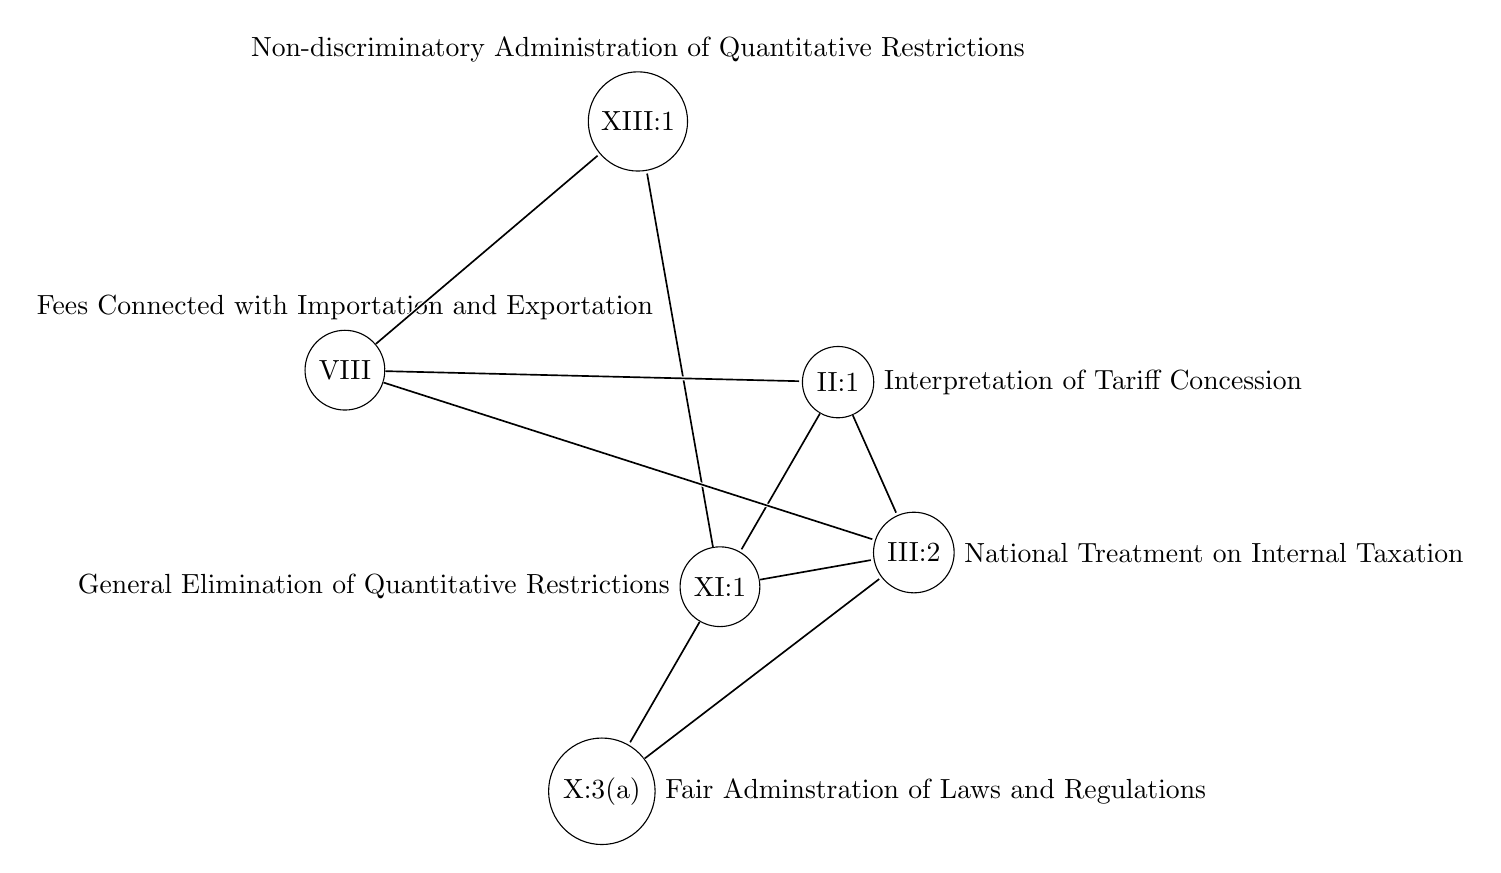
\begin{tikzpicture}[>={Stealth[color=black]},shorten >=1pt,node distance=2cm,on grid,initial/.style={}]
        \node[state, label=right:Interpretation of Tariff Concession] (T1) {II:1};
        \node[state, label=left:General Elimination of Quantitative Restrictions] at ([shift=({240:3cm})]T1) (T4) {XI:1};
        \node[state, label=right:Fair Adminstration of Laws and Regulations] at ([shift=({240:3 cm})]T4) (T5) {X:3(a)};
        \node[state, label=above:Non-discriminatory Administration of Quantitative Restrictions] at ([shift=({100:6 cm})]T4) (T7) {XIII:1};
        \node[state, label=right:National Treatment on Internal Taxation] at ([shift=({10:2.5 cm})]T4) (T6) {III:2};
        \node[state, label=above:Fees Connected with Importation and Exportation] at ([shift=({150:5.5 cm})]T4) (T8) {VIII};
        
        \begin{scope}[every edge/.append style={-, double=black, draw=white}] % for directed edge, change "style={->, double=black, draw=white}]"
          \path (T1)
          edge   (T4)
          edge   (T6);
          \path (T4)
          edge   (T5)
          edge   (T6)
          edge   (T7);
          \path (T5)
          edge   (T6);
          \path (T8)
          edge   (T7)
          edge   (T1)
          edge   (T6);
        \end{scope}

        % \draw[line width=0.1pt,red,double=red,double distance=1pt] (T6) -- (T4); %III:2, XI:1
        % \draw[line width=0.1pt,magenta,double=black,double distance=1pt] (T1) -- (T6); % II:1 III:2 
        % \draw[line width=1pt,black,double=black,double distance=1pt] (T1) -- (T4); % II:1 III:2

      \end{tikzpicture}
    }
    \caption{Market Access}
    \label{fig:market-aceess}
  \end{figure}
  

  % XI:1 <-> III:2 :: 0.232
  % II:1 <-> III:2 :: 0.2385
%  ------
  % II:1 <-> XI:1 :: 0.19
  % X:3(a) <-> III:2 :: 0.196
  % X:3(a) <-> X:3(a) :: 0.184
 % ------
  % VIII <-> II:1 :: 0.167
  % XI:1 <-> XIII:1 :: 0.169
  %-----
  % VIII <-> III:2 :: 0.138
  % VIII <-> II:1 :: 0.138
  %----


\section{Conclusion}
This paper shows how WTO works.

\begin{itemize}
  \item Implicaiton of thie method in general.
  \item Address the imbalance of legal capacity between developed/ing countries
\end{itemize}

\clearpage

\bibliography{bibtemplate}

\clearpage
\begin{appendices}
\section{}
\label{sec:appendix}
% \subsection{Table of Contents of the Panel Report}
% \begin{figure}[h]
    \centering
    \includegraphics[scale=0.3]{Data/pngs/panel_report_toc.png}
    \caption{{\bf Table of Contents of the Panel Report}}
    % : }It shows {\bf II. FACTUAL ASPECTS}
\end{figure}

% \begin{center}
%     \includegraphics[scale=0.3]{Data/pngs/panel_report_toc.png}
% \end{center}



\subsection{Factual Aspect Example}
\label{sub:factual-aspect-example}
Excerpt below is from the panel report for the 
\textit{US - Offset Act (Byrd Amendment)}
\footnote{Panel Report, United States — Continued Dumping and Subsidy Offset Act of 2000, WTO Doc. WT/DS217/R (adopted Jan. 27, 2003).} case.\\

\begin{tcolorbox}[breakable]
\noindent{\bf II. FACTUAL ASPECTS}\\\\
2.1 \quad This dispute concerns the Continued Dumping and Subsidy Offset Act of 2000 (the
“CDSOA” or the “Offset Act”), which was enacted on 28 October 2000 as part of the Agriculture,
Rural Development, Food and Drug Administration and Related Agencies Appropriations Act, 2001.1
The CDSOA amends Title VII of the Tariff Act of 1930 by adding a new section 754 entitled
Continued Dumping and Subsidy Offset. Regulations prescribing administrative procedures under the
Act were brought into effect on September 21, 2001.\\

\noindent2.2 \quad The CDSOA provides that :

\blockquote{
    Duties assessed pursuant to a countervailing duty order, an anti-dumping duty order,
    or a finding under the Antidumping Act of 1921 shall be distributed on an annual
    basis under this section to the affected domestic producers for qualifying
    expenditures. Such distribution shall be known as “the continued dumping and
    subsidy offset”.
    }
\\\\
\noindent2.3 \quad The term “affected domestic producers” means :

\blockquote{
    a manufacturer, producer, farmer, rancher, or worker representative (including
associations of such persons) that – \\\\
        (A) was a petitioner or interested party in support of the petition with respect
to which an anti-dumping duty order, a finding under the Antidumping Act of 1921,
or a countervailing duty order has been entered, and \\\\
\quad \quad (B) remains in operation. \\\\
Companies, business, or persons that have ceased the production of the product
covered by the order or finding or who have been acquired by a company or business
that is related to a company that opposed the investigation shall not be an affected
domestic producer.
}
\\\\
\noindent 2.4 \quad In turn, the term “qualifying expenditure” is defined by the CDSOA as “expenditure[s]
incurred after the issuance of the anti-dumping duty finding or order or countervailing duty order in
any of the following categories:
\blockquote{\\
(A) Manufacturing facilities.\\
(B) Equipment.\\
(C) Research and development.\\
(D) Personnel training.\\
(E) Acquisition of technology.\\
(F) Health care benefits to employees paid for by the employer.\\
(G) Pension benefits to employees paid for by the employer.\\
(H) Environmental equipment, training or technology.\\
(I) Acquisition of raw materials and other inputs.\\
(J) Working capital or other funds needed to maintain production.”
}
\\\\
\noindent 2.5 \quad The CDSOA provides that the Commissioner of Customs shall establish in the Treasury of
the United States a special account with respect to each order or finding8
 and deposit into such
account all the duties assessed under that Order.9
 The Commissioner of Customs shall distribute all
funds (including all interest earned on the funds) from the assessed duties received in the preceding
fiscal year to affected domestic producers based on a certification by the affected domestic producer
that he is eligible to receive the distribution and desires to receive a distribution for qualifying
expenditures incurred since the issuance of the order or finding.10 Funds deposited in each special
account during each fiscal year are to be distributed no later than 60 days after the beginning of the
following fiscal year.11 The CDSOA and regulations prescribe that (1) if the total amount of the
certified net claims filed by affected domestic producers does not exceed the amount of the offset
available, the certified net claim for each affected domestic producer will be paid in full, and (2) if the
certified net claims exceed the amount available, the offset will be made on a pro rata basis based on
each affected domestic producer’s total certified claim.\\

\noindent 2.6 \quad Special accounts are to be terminated after “(A) the order or finding with respect to which the
account was established has terminated; (B) all entries relating to the order or finding are liquidated
and duties assessed collected; (C) the Commissioner has provided notice and a final opportunity to
obtain distribution pursuant to subsection (c); and (D) 90 days has elapsed from the date of the notice
described in subparagraph (C).” All amounts that remain unclaimed in the Account are to be
permanently deposited into the general fund in the US Treasury.12\\

\noindent 2.7 \quad The CDSOA applies with respect to all anti-dumping and countervailing duty assessments
made on or after 1 October 200013 pursuant to an anti-dumping order or a countervailing order or a
finding under the Antidumping Act of 1921 in effect on 1 January 1999 or issued thereafter. [END]

\end{tcolorbox}

\subsection{Collected Cited Articles for 143 WTO DSB Cases}
DS refers to \textit{Dispute Settelement} and this notation is officially adopted by WTO DSB.\\
WTO DSB identifies each dispute with a unique number for each case such as DS2 and DS18.
\label{sub:cited-articles-table}

\begin{xltabular}{\linewidth}{ l | X }
    % \caption{Description of Variables used in this Study}
    % \label{table: vardescription}
    \hline 

    \textbf{\normalsize DS} & \textbf{\normalsize Articles Cited}  \\
    \endfirsthead
    \hline \hline

    \textbf{DS2} & I, II:1(b) \\ \hline

    \textbf{DS3} & I, II:1(b) \\ \hline

    \textbf{DS2} & I, II:1(b) \\ \hline

    \textbf{DS3} & I, II:1(b) \\ \hline

    \textbf{DS2} & I, II:1(b) \\ \hline

    \textbf{DS3} & I, II:1(b) \\ \hline

    \textbf{DS2} & I, II:1(b) \\ \hline

    \textbf{DS3} & I, II:1(b) \\ \hline

    \textbf{DS2} & I, II:1(b) \\ \hline

    \textbf{DS3} & I, II:1(b) \\ \hline

    \textbf{DS2} & I, II:1(b) \\ \hline

    \textbf{DS3} & I, II:1(b) \\ \hline

    \textbf{DS2} & I, II:1(b) \\ \hline

    \textbf{DS3} & I, II:1(b) \\ \hline

    \textbf{DS2} & I, II:1(b) \\ \hline

    \textbf{DS3} & I, II:1(b) \\ \hline

    \textbf{DS2} & I, II:1(b) \\ \hline

    \textbf{DS3} & I, II:1(b) \\ \hline

    \textbf{DS2} & I, II:1(b) \\ \hline

    \textbf{DS3} & I, II:1(b) \\ \hline

    \textbf{DS2} & I, II:1(b) \\ \hline

    \textbf{DS3} & I, II:1(b) \\ \hline

    \textbf{DS2} & I, II:1(b) \\ \hline

    \textbf{DS3} & I, II:1(b) \\ \hline

    \textbf{DS2} & I, II:1(b) \\ \hline

    \textbf{DS3} & I, II:1(b) \\ \hline

    \textbf{DS2} & I, II:1(b) \\ \hline

    \textbf{DS3} & I, II:1(b) \\ \hline

    \textbf{DS2} & I, II:1(b) \\ \hline

    \textbf{DS3} & I, II:1(b) \\ \hline

    \textbf{DS2} & I, II:1(b) \\ \hline

    \textbf{DS3} & I, II:1(b) \\ \hline

    \textbf{DS2} & I, II:1(b) \\ \hline

    \textbf{DS3} & I, II:1(b) \\ \hline

    \textbf{DS2} & I, II:1(b) \\ \hline

    \textbf{DS3} & I, II:1(b) \\ \hline

    \textbf{DS2} & I, II:1(b) \\ \hline

    \textbf{DS3} & I, II:1(b) \\ \hline

    \textbf{DS2} & I, II:1(b) \\ \hline

    \textbf{DS3} & I, II:1(b) \\ \hline

    \textbf{DS2} & I, II:1(b) \\ \hline

    \textbf{DS3} & I, II:1(b) \\ \hline

    \textbf{DS2} & I, II:1(b) \\ \hline

    \textbf{DS3} & I, II:1(b) \\ \hline

    \textbf{DS2} & I, II:1(b) \\ \hline

    \textbf{DS3} & I, II:1(b) \\ \hline

    \textbf{DS2} & I, II:1(b) \\ \hline

    \textbf{DS3} & I, II:1(b) \\ \hline

    \textbf{DS2} & I, II:1(b) \\ \hline

    \textbf{DS3} & I, II:1(b) \\ \hline

    \textbf{DS2} & I, II:1(b) \\ \hline

    \textbf{DS3} & I, II:1(b) \\ \hline

    \textbf{DS2} & I, II:1(b) \\ \hline

    \textbf{DS3} & I, II:1(b) \\ \hline

    \textbf{DS2} & I, II:1(b) \\ \hline

    \textbf{DS3} & I, II:1(b) \\ \hline

    \textbf{DS2} & I, II:1(b) \\ \hline

    \textbf{DS3} & I, II:1(b) \\ \hline

    \textbf{DS2} & I, II:1(b) \\ \hline

    \textbf{DS3} & I, II:1(b) \\ \hline

    \textbf{DS2} & I, II:1(b) \\ \hline

    \textbf{DS3} & I, II:1(b) \\ \hline

    \textbf{DS2} & I, II:1(b) \\ \hline

    \textbf{DS3} & I, II:1(b) \\ \hline

    \textbf{DS2} & I, II:1(b) \\ \hline

    \textbf{DS3} & I, II:1(b) \\ \hline

    \textbf{DS2} & I, II:1(b) \\ \hline

    \textbf{DS3} & I, II:1(b) \\ \hline

    \textbf{DS2} & I, II:1(b) \\ \hline

    \textbf{DS3} & I, II:1(b) \\ \hline

    \textbf{DS2} & I, II:1(b) \\ \hline

    \textbf{DS3} & I, II:1(b) \\ \hline

    \textbf{DS2} & I, II:1(b) \\ \hline

    \textbf{DS3} & I, II:1(b) \\ \hline

    \textbf{DS2} & I, II:1(b) \\ \hline

    \textbf{DS3} & I, II:1(b) \\ \hline

    \textbf{DS2} & I, II:1(b) \\ \hline

    \textbf{DS3} & I, II:1(b) \\ \hline

    \textbf{DS2} & I, II:1(b) \\ \hline

    \textbf{DS3} & I, II:1(b) \\ \hline

    \textbf{DS2} & I, II:1(b) \\ \hline

    \textbf{DS3} & I, II:1(b) \\ \hline

    \textbf{DS2} & I, II:1(b) \\ \hline

    \textbf{DS3} & I, II:1(b) \\ \hline

    \textbf{DS2} & I, II:1(b) \\ \hline

    \textbf{DS3} & I, II:1(b) \\ \hline

    \textbf{DS2} & I, II:1(b) \\ \hline

    \textbf{DS3} & I, II:1(b) \\ \hline

    \textbf{DS2} & I, II:1(b) \\ \hline

    \textbf{DS3} & I, II:1(b) \\ \hline

    \textbf{DS2} & I, II:1(b) \\ \hline

    \textbf{DS3} & I, II:1(b) \\ \hline

    \textbf{DS2} & I, II:1(b) \\ \hline

    \textbf{DS3} & I, II:1(b) \\ \hline

    \textbf{DS2} & I, II:1(b) \\ \hline

    \textbf{DS3} & I, II:1(b) \\ \hline

    \textbf{DS2} & I, II:1(b) \\ \hline

    \textbf{DS3} & I, II:1(b) \\ \hline

    \textbf{DS2} & I, II:1(b) \\ \hline

    \textbf{DS3} & I, II:1(b) \\ \hline

    \textbf{DS2} & I, II:1(b) \\ \hline

    \textbf{DS3} & I, II:1(b) \\ \hline

    \textbf{DS2} & I, II:1(b) \\ \hline

    \textbf{DS3} & I, II:1(b) \\ \hline

    \textbf{DS2} & I, II:1(b) \\ \hline

    \textbf{DS3} & I, II:1(b) \\ \hline

    \textbf{DS2} & I, II:1(b) \\ \hline

    \textbf{DS3} & I, II:1(b) \\ \hline

    \textbf{DS2} & I, II:1(b) \\ \hline

    \textbf{DS3} & I, II:1(b) \\ \hline

    \textbf{DS2} & I, II:1(b) \\ \hline

    \textbf{DS3} & I, II:1(b) \\ \hline

    \textbf{DS2} & I, II:1(b) \\ \hline

    \textbf{DS3} & I, II:1(b) \\ \hline

    \textbf{DS2} & I, II:1(b) \\ \hline

    \textbf{DS3} & I, II:1(b) \\ \hline

    \textbf{DS2} & I, II:1(b) \\ \hline

    \textbf{DS3} & I, II:1(b) \\ \hline

    \textbf{DS2} & I, II:1(b) \\ \hline

    \textbf{DS3} & I, II:1(b) \\ \hline

    \textbf{DS2} & I, II:1(b) \\ \hline

    \textbf{DS3} & I, II:1(b) \\ \hline

    \textbf{DS2} & I, II:1(b) \\ \hline

    \textbf{DS3} & I, II:1(b) \\ \hline

    \textbf{DS2} & I, II:1(b) \\ \hline

    \textbf{DS3} & I, II:1(b) \\ \hline

    \textbf{DS2} & I, II:1(b) \\ \hline

    \textbf{DS3} & I, II:1(b) \\ \hline

    \textbf{DS2} & I, II:1(b) \\ \hline

    \textbf{DS3} & I, II:1(b) \\ \hline

    \textbf{DS2} & I, II:1(b) \\ \hline

    \textbf{DS3} & I, II:1(b) \\ \hline

    \textbf{DS2} & I, II:1(b) \\ \hline

    \textbf{DS3} & I, II:1(b) \\ \hline

    \textbf{DS2} & I, II:1(b) \\ \hline

    \textbf{DS3} & I, II:1(b) \\ \hline

    \textbf{DS2} & I, II:1(b) \\ \hline

    \textbf{DS3} & I, II:1(b) \\ \hline

    \textbf{DS2} & I, II:1(b) \\ \hline

    \textbf{DS3} & I, II:1(b) \\ \hline

    \textbf{DS2} & I, II:1(b) \\ \hline

    \textbf{DS3} & I, II:1(b) \\ \hline

    \textbf{DS2} & I, II:1(b) \\ \hline \hline

\end{xltabular}

\subsection{Technical Details}
\label{sub:technicial-details}

% == HEATMAP MATRIX == 
\begin{figure}[!tbp]
    \begin{subfigure}[b]{0.49\textwidth}
      \centering{
        \resizebox{\textwidth*\real{\heatmap}}{\textwidth*\real{\heatmap} * \real{1.7889}}{% \begin{figure}[h]
%     \centering
    \begin{tikzpicture}
        \foreach \i in {\xMin,...,5} {
            \draw [black] (\i,4) -- (\i,9) node [below] at (\i,4) {};
        }
        \foreach \i in {4,...,9} {
            \draw [black] (\xMin,\i) -- (5,\i) node [left] at (\xMin,\i) {};
        }

        % \node [left] at (0,0.5) {\textbf{XXVIII}};
        % \node [left] at (0,1.5) {\textbf{XXVI:6}};
        % \node [left] at (0,2.5) {\textbf{XXIV:5(b)}};
        % \node [left] at (0,3.5) {\textbf{XXIV:12}};
        \node [left] at (0,4.5) {\textbf{\vdots}};
        \node [left] at (0,5.5) {\textbf{II:1}};
        \node [left] at (0,6.5) {\textbf{II}};
        \node [left] at (0,7.5) {\textbf{I:1}};
        \node [left] at (0,8.5) {\textbf{I}};

        % \node [left] at (8.8, 9.25) {\textbf{XXVIII}};
        % \node [left] at (7.8, 9.25) {\textbf{XXVI:6}};
        % \node [left] at (6.8, 9.25) {\textbf{XXIV:5(b)}};
        % \node [left] at (5.8, 9.25) {\textbf{XXIV:12}};
        \node [left] at (4.8, 9.25) {\textbf{\ldots}};
        \node [left] at (3.8, 9.25) {\textbf{II:1}};
        \node [left] at (2.8, 9.25) {\textbf{II}};
        \node [left] at (1.85, 9.25) {\textbf{I:1}};
        \node [left] at (0.7,9.25) {\textbf{I}};

        \node [left] at (0.7,8.5) {\textbf{0}};
        \node [left] at (1.7,8.5) {\textbf{3}};
        \node [left] at (2.8,8.5) {\textbf{7}};
        \node [left] at (3.8,8.5) {\textbf{2}};
        
        \node [left] at (0.7,7.5) {\textbf{3}};
        \node [left] at (1.7,7.5) {\textbf{0}};
        \node [left] at (2.8,7.5) {\textbf{3}};
        \node [left] at (3.8,7.5) {\textbf{4}};

        \node [left] at (0.7,6.5) {\textbf{7}};
        \node [left] at (1.7,6.5) {\textbf{3}};
        \node [left] at (2.8,6.5) {\textbf{0}};
        \node [left] at (3.8,6.5) {\textbf{4}};

        \node [left] at (0.7,5.5) {\textbf{2}};
        \node [left] at (1.7,5.5) {\textbf{4}};
        \node [left] at (2.8,5.5) {\textbf{4}};
        \node [left] at (3.8,5.5) {\textbf{0}};



        % \node [left] at (5.5,9.5) {\textbf{Embedding Dimension = $k$}};
        % \node [right, rotate=-90, font=\small] at (6.5,7) {\textbf{Max Sequence Length = $n$}};


    % \draw [step=1.0,blue, very thick] (0.5,0.5) grid (5.5,4.5);
    % \draw [very thick, brown, step=1.0cm,xshift=-0.5cm, yshift=-0.5cm] (0.5,0.5) grid +(5.5,4.5);
    \end{tikzpicture} 
%     \label{fig:visualize-co-cites}      
%     \caption{\textbf{Definition of Co-citation Matrix:} This paper defines co-citation matrix $C$ as a $\mid V \mid \times \mid V \mid$ matrix where each element $c_{ij}:= \text{Counts of } $ is count of all co-occurrence $  \text{ } s.t. \text{ } \forall i,j \in \mid V \mid$ } 
% \end{figure}

% This  dispute  concerns  the  Continued  Dumping }
        \caption{Co-citation}
        \label{sparse_matrix}
      }
    \end{subfigure}
    \hfill
    \begin{subfigure}[b]{0.49\textwidth}
      \centering{
        \resizebox{\textwidth*\real{\heatmap}}{\textwidth*\real{\heatmap} * \real{1.7889}}{\input{pred.tex}}
        \caption{Prediction}
        \label{predidction_matrix}
      }
    \end{subfigure}
    \caption{{\bf Co-citation \& Prediction}}
    \label{sparse_dense}
  \end{figure}
  

% % This file was created by tikzplotlib v0.9.4.
\begin{tikzpicture}

\begin{axis}[
tick align=outside,
tick pos=left,
title={coo},
x grid style={white!69.0196078431373!black},
xmin=0, xmax=58,
xtick style={color=black},
y grid style={white!69.0196078431373!black},
ymin=0, ymax=58,
ytick style={color=black}
]
\addplot graphics [includegraphics cmd=\pgfimage,xmin=0, xmax=58, ymin=0, ymax=58] {coo-001.png};
\end{axis}

\end{tikzpicture}

\end{appendices}
% == END
\end{document}